\documentclass[tikz,border=10pt]{standalone}
\usepackage{helvet}
\usepackage{amsmath,amssymb}
\renewcommand{\familydefault}{\sfdefault}
\usetikzlibrary{shapes.geometric, arrows.meta, positioning, calc, fit, backgrounds}

\begin{document}
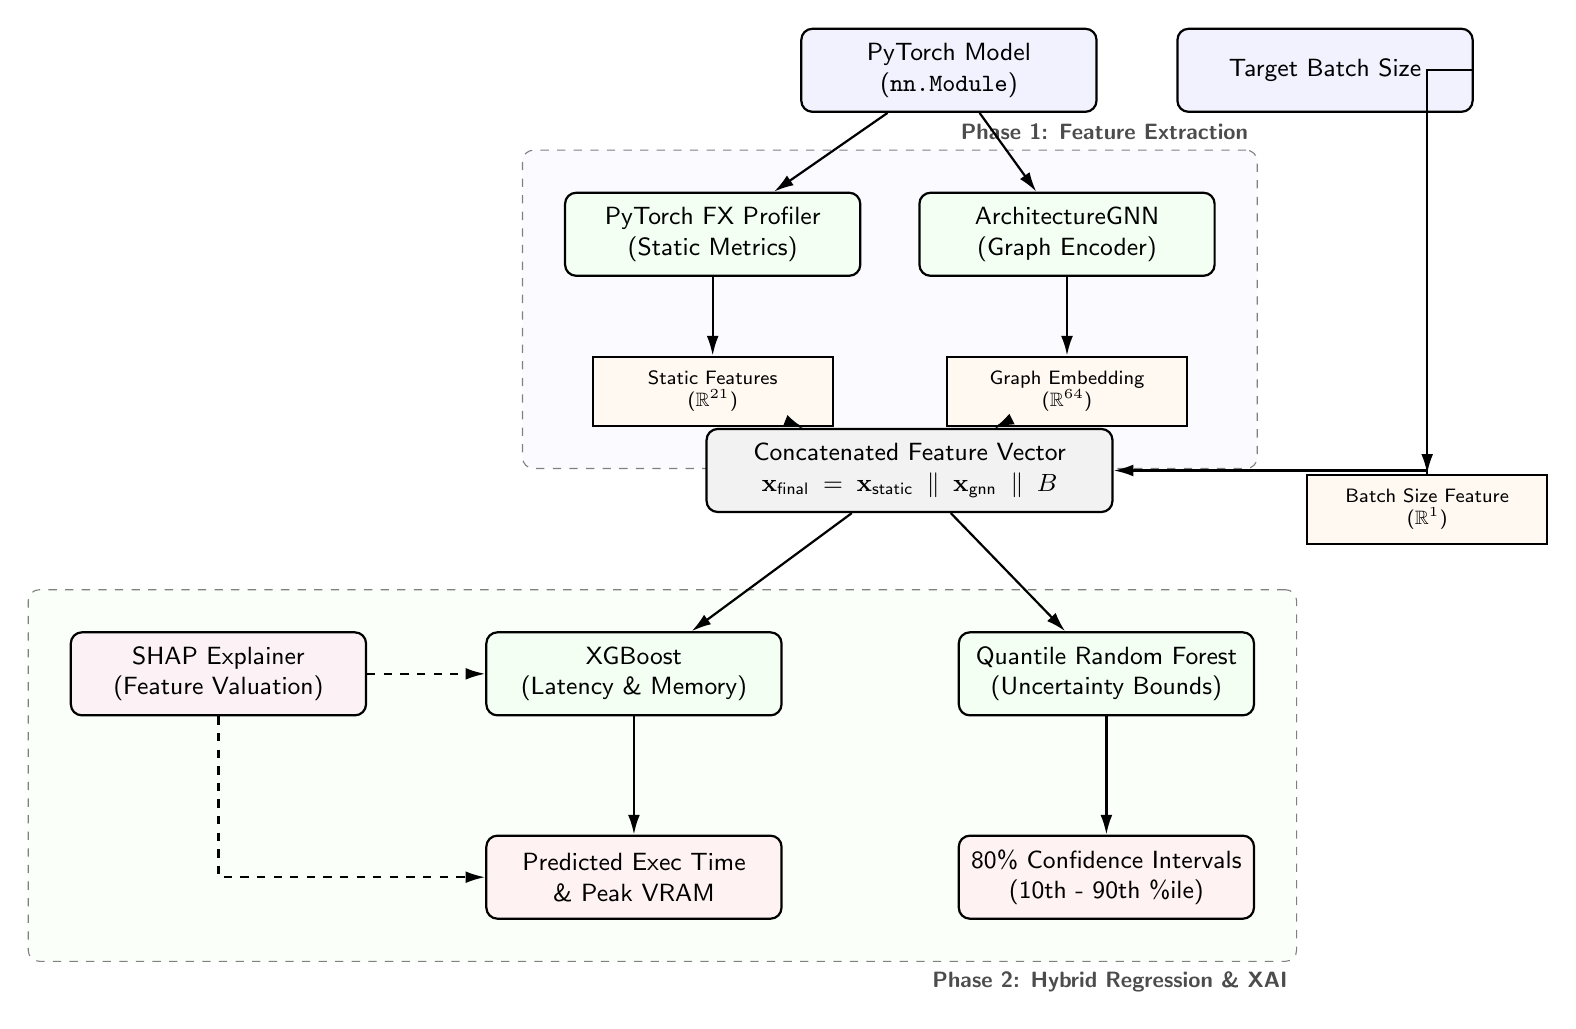
\begin{tikzpicture}[
    auto,
    node distance=1.5cm and 2cm,
    block/.style = {rectangle, draw=black, thick, fill=blue!5, text width=10em, text centered, rounded corners, minimum height=3em, font=\small},
    model/.style = {rectangle, draw=black, thick, fill=green!5, text width=10em, text centered, rounded corners, minimum height=3em, font=\small},
    feature/.style = {rectangle, draw=black, thick, fill=orange!5, text width=8em, text centered, minimum height=2.5em, font=\scriptsize},
    output/.style = {rectangle, draw=black, thick, fill=red!5, text width=10em, text centered, rounded corners, minimum height=3em, font=\small},
    line/.style = {draw, thick, -{Latex[length=2.5mm,width=1.5mm]}},
]

% Inputs
\node [block] (input) {PyTorch Model (\texttt{nn.Module})};
\node [block, right=1cm of input] (batch) {Target Batch Size};

% Feature Extractors
\node [model, below=1cm of input, xshift=-3cm] (static) {PyTorch FX Profiler\\(Static Metrics)};
\node [model, below=1cm of input, xshift=1.5cm] (gnn) {ArchitectureGNN\\(Graph Encoder)};

% Feature Vectors
\node [feature, below=1cm of static] (f_static) {Static Features\\($\mathbb{R}^{21}$)};
\node [feature, below=1cm of gnn] (f_gnn) {Graph Embedding\\($\mathbb{R}^{64}$)};

\node [feature, right=1.5cm of f_gnn, yshift=-1.5cm] (f_batch) {Batch Size Feature\\($\mathbb{R}^{1}$)};

% Concatenation
\node [block, fill=gray!10, text width=14em, below=4cm of input, xshift=-0.5cm] (concat) {Concatenated Feature Vector\\$\mathbf{x}_{\text{final}} = \mathbf{x}_{\text{static}} \parallel \mathbf{x}_{\text{gnn}} \parallel B$};

% Predictors
\node [model, below=1.5cm of concat, xshift=-3.5cm] (xgb) {XGBoost\\(Latency \& Memory)};
\node [model, below=1.5cm of concat, xshift=2.5cm] (rf) {Quantile Random Forest\\(Uncertainty Bounds)};

% Outputs
\node [output, below=1.5cm of xgb] (out_primary) {Predicted Exec Time \& Peak VRAM};
\node [output, below=1.5cm of rf] (out_bounds) {80\% Confidence Intervals\\(10th - 90th \%ile)};

% SHAP Explainer
\node [block, fill=purple!5, left=1.5cm of xgb] (shap) {SHAP Explainer\\(Feature Valuation)};

% Paths
\path [line] (input) -- (static);
\path [line] (input) -- (gnn);
\path [line] (static) -- (f_static);
\path [line] (gnn) -- (f_gnn);
\path [line] (batch) -| (f_batch);

\path [line] (f_static) -- (concat);
\path [line] (f_gnn) -- (concat);
\path [line] (f_batch) |- (concat);

\path [line] (concat) -- (xgb);
\path [line] (concat) -- (rf);

\path [line] (xgb) -- (out_primary);
\path [line] (rf) -- (out_bounds);

\path [line, dashed] (shap) -- (xgb);
\path [line, dashed] (shap) |- (out_primary);


% Background Boxes (Visual Grouping)
\begin{scope}[on background layer]
    % Extraction Phase
    \node[draw=black!50, dashed, inner sep=15pt, fit=(static) (gnn) (f_static) (f_gnn), fill=blue!2, rounded corners] (box1) {};
    \node[anchor=south east, text=black!70, font=\footnotesize\bfseries] at (box1.north east) {Phase 1: Feature Extraction};
    
    % Regression Phase
    \node[draw=black!50, dashed, inner sep=15pt, fit=(xgb) (rf) (shap) (out_primary) (out_bounds), fill=green!2, rounded corners] (box2) {};
    \node[anchor=north east, text=black!70, font=\footnotesize\bfseries] at (box2.south east) {Phase 2: Hybrid Regression \& XAI};
\end{scope}

\end{tikzpicture}
\end{document}
